\documentclass[11pt]{amsart}
\usepackage{geometry}                % See geometry.pdf to learn the layout options. There are lots.
\geometry{letterpaper}                   % ... or a4paper or a5paper or ... 
%\geometry{landscape}                % Activate for for rotated page geometry
%\usepackage[parfill]{parskip}    % Activate to begin paragraphs with an empty line rather than an indent
\usepackage{graphicx}
\usepackage{amssymb}
\usepackage{epstopdf}
\usepackage{caption}
\usepackage{subcaption}
\DeclareGraphicsRule{.tif}{png}{.png}{`convert #1 `dirname #1`/`basename #1 .tif`.png}

% Declare commands
\newcommand{\mat}[1]{\mathbf{#1}}

\title{CS 181 -- Practical 1}
\author{Casey Grun, Sam Kim, Rhed Shi}
%\date{}                                           % Activate to display a given date or no date

\begin{document}
\maketitle

\section{Warmup}
We used the K-Means algorithm to cluster the images of the CIFAR-10 dataset, which consists of 60000 total 32x32 color images. We only clustered a single batch, consisting of 10000 images. The algorithm was run for $k=5,10,15$.\\
The following sets of images show the mean images of the k clusters for $k=5,10,15$ as well as the 25 images that are closest to each of the respective means for $k=5,10$.\\

\begin{figure}[h]
	\centering
	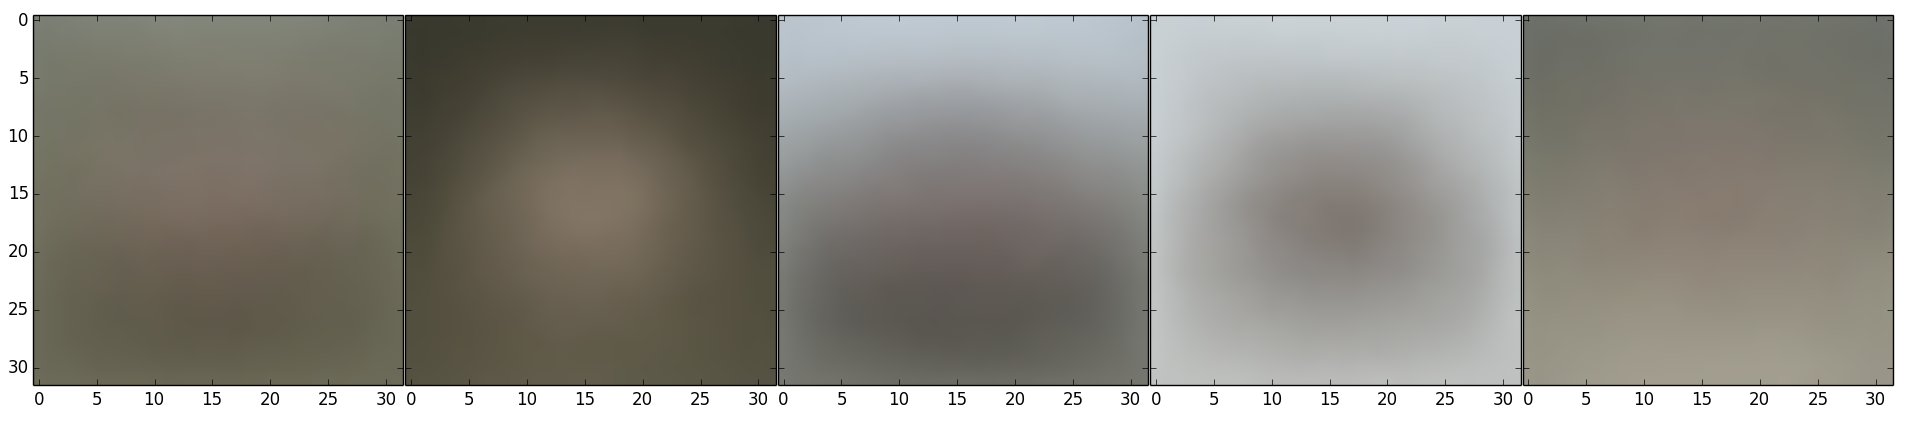
\includegraphics[width=8cm]{images/k5us.png}\\
	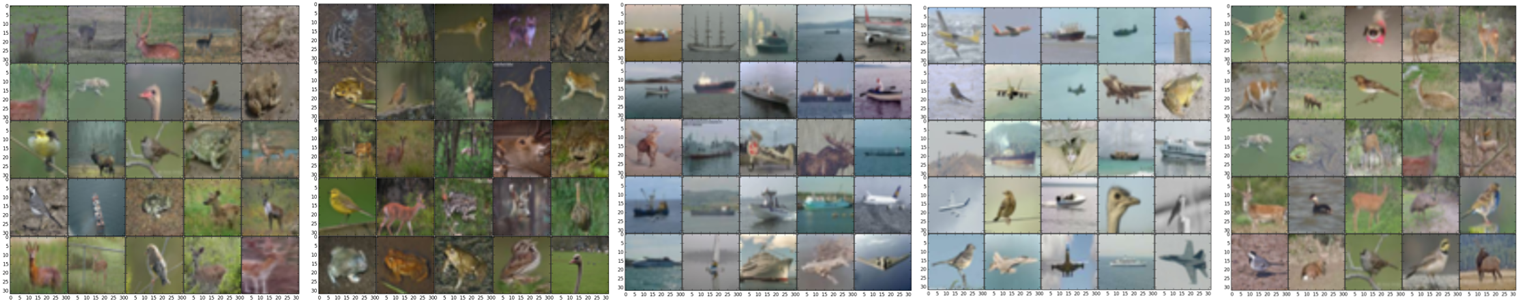
\includegraphics[width=15cm]{images/k5reps.png}\\
	\caption{(Top) Cluster means and (bottom) 25 representative images for each of the cluster means for $k=5$.}
\end{figure}

\begin{figure}[h]
	\centering
	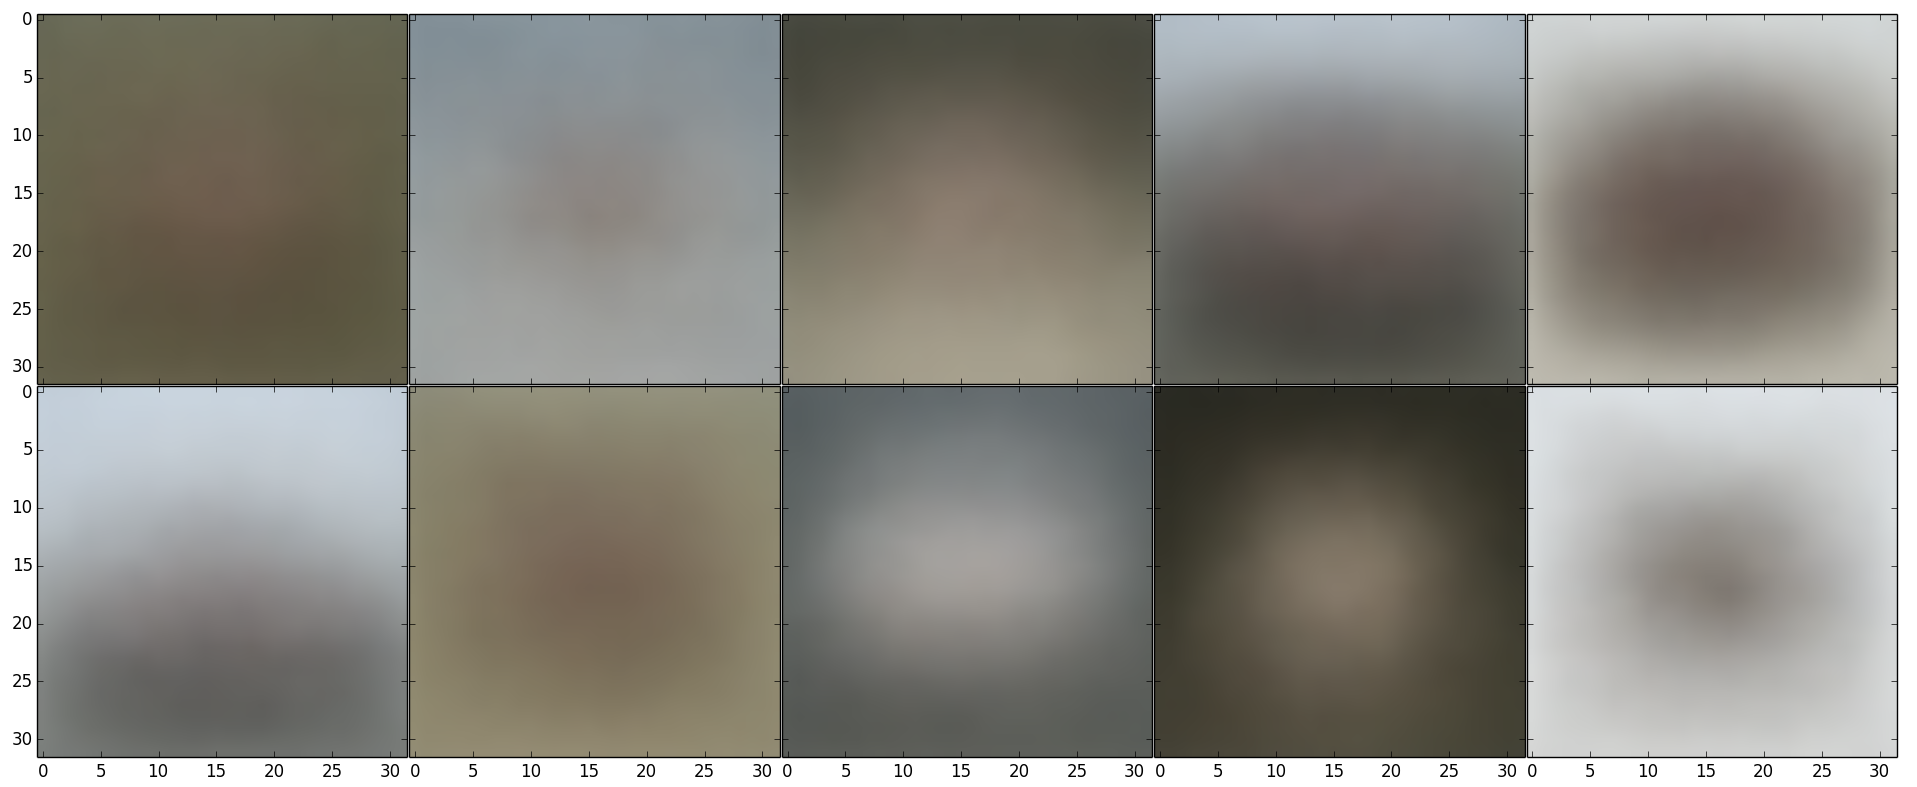
\includegraphics[width=8cm]{images/k10us.png}\\
	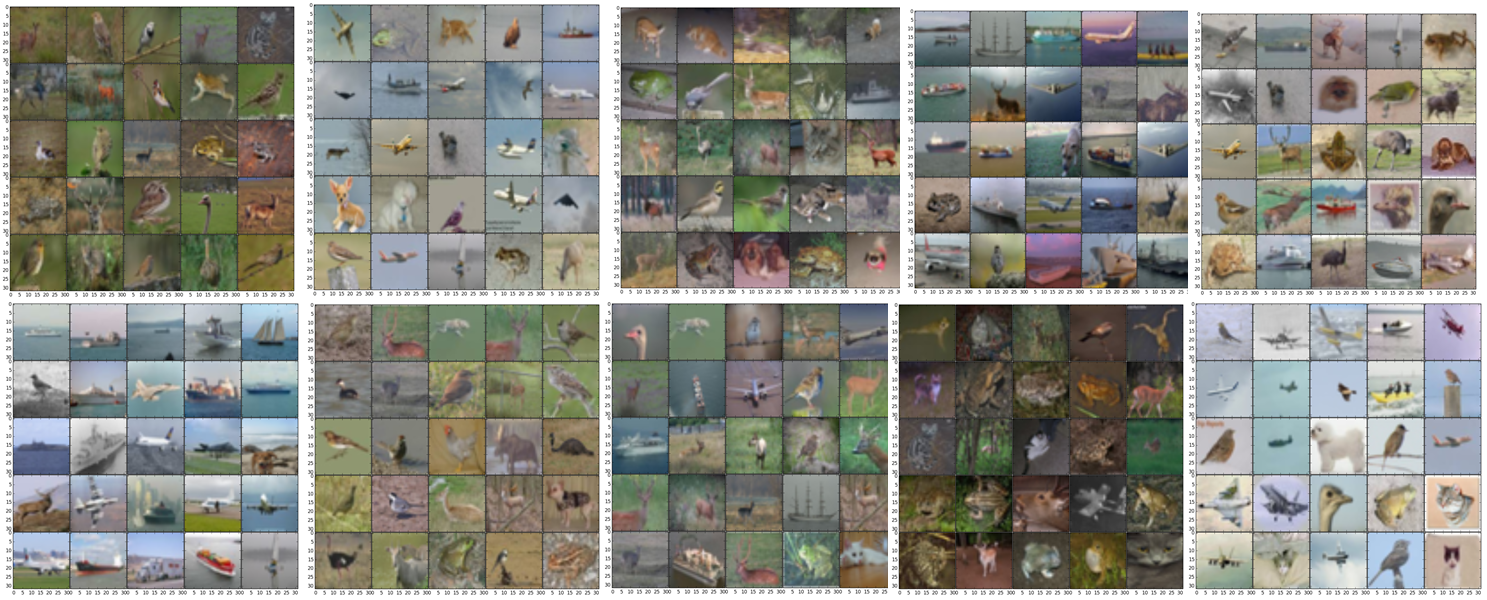
\includegraphics[width=15cm]{images/k10reps.png}\\
	\caption{(Top) Cluster means and (bottom) 25 representative images for each of the cluster means for $k=10$.}
\end{figure}

\begin{figure}
\centering
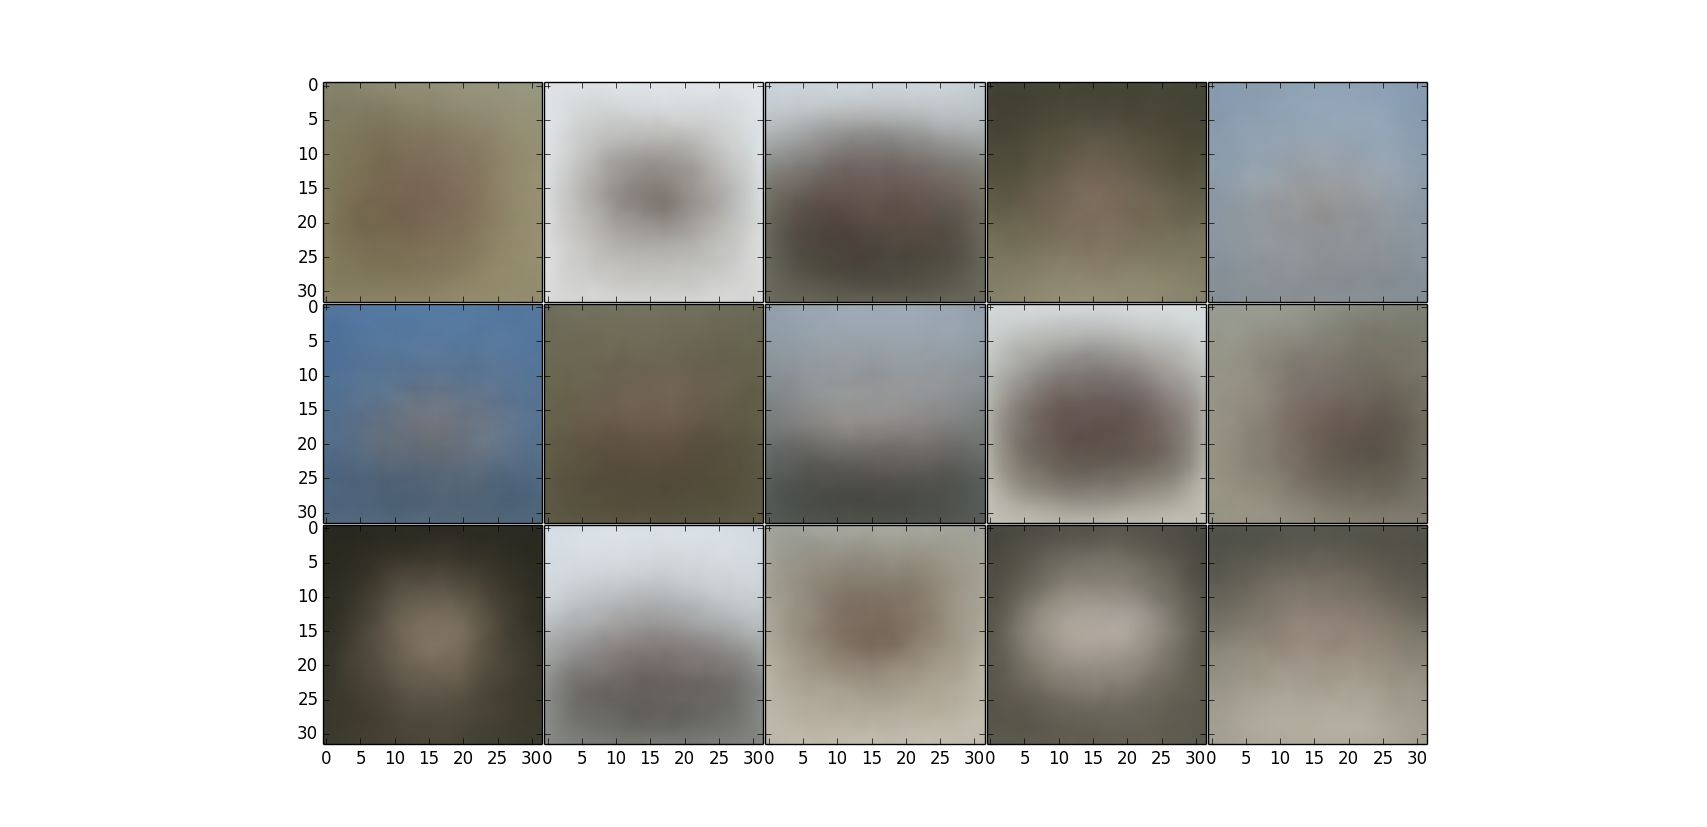
\includegraphics[width=7cm]{images/k15us.png}
\caption{Cluster means for $k=15$}
\end{figure}

Although features are not discernible from the mean images, there are still trends of lighter colors versus darker colors, which is consistent with the representative images. For example, in $k=5$, the 2nd cluster mean is mostly dark around the edges whereas the 4th cluster mean is mostly light around the edges, and the representative images share these features. Additionally, we see that as we increase $k$, the distinction between mean images increase as well. For $k=5$, the means are mostly greyish brown images, whereas for $k=15$, several of the mean images have tints of blue.\\

We use the objective function:
$$J(\{r_n\}^N_{n=1},\{\mu_k\}^K_{k=1})=\sum^N_{n=1}\sum^K_{k=1}r_{nk}||x_n-\mu_k||^2_2$$
where $r_n$ is the responsibilities vector of the $n$th data point, $\mu_k$ is the mean of the $k$th cluster, and $x_n$ is the $n$th data point. Plots of the objective function as a function of iteration for $k=5,10,15$ are shown below.


\begin{figure}[h]
	\centering
	\begin{subfigure}{0.5\textwidth}
		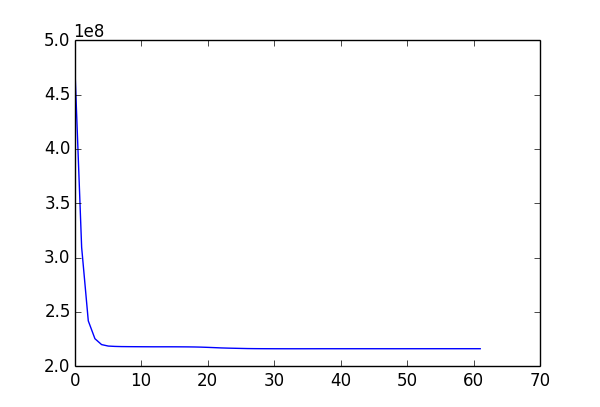
\includegraphics[width=7cm]{images/k5objectives.png}
		\caption{$k=5$}
	\end{subfigure}
	\begin{subfigure}{0.3\textwidth}
		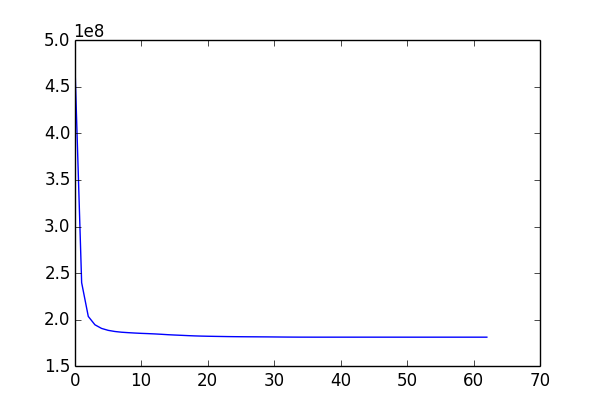
\includegraphics[width=7cm]{images/k10objectives.png}
		\caption{$k=10$}
	\end{subfigure}
	\begin{subfigure}{0.3\textwidth}
		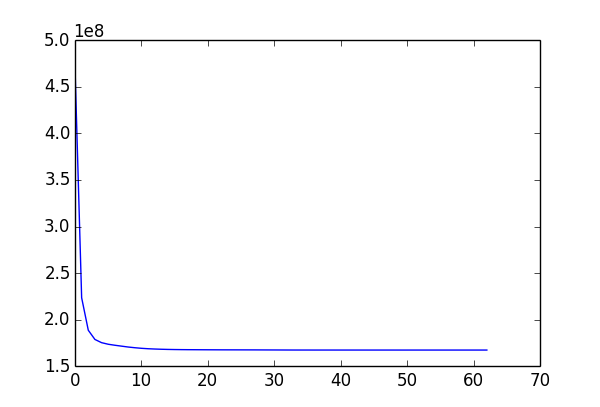
\includegraphics[width=7cm]{images/k15objectives.png}
		\caption{$k=15$}
	\end{subfigure}
	\caption{Objective function as a function of iteration for K-Means}
\end{figure}

We can see that for all 3 $k$s, the objective function never increases over the iteration, so the algorithm is constantly finding a better solution and converging to a (local) minimum. In addition, comparing the objective functions, $k=5$ reaches approximately $J=2.2\times 10^{8}$, $k=10$ converges to $J=1.8\times 10^{8}$, and $k=15$ converges to $J=1.7\times 10^{8}$. As suspected, allowing more clusters allows the images to be closer to their respective cluster means.\\

\begin{figure}[h]
	\centering
	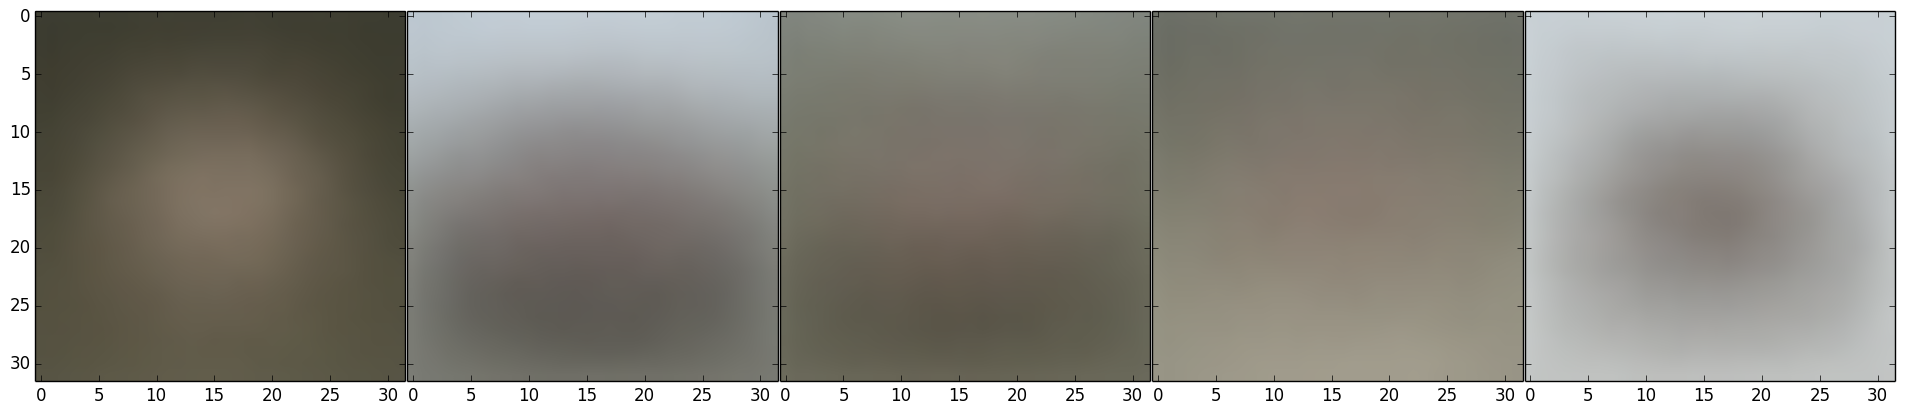
\includegraphics[width=8cm]{images/kplus5us.png}\\
	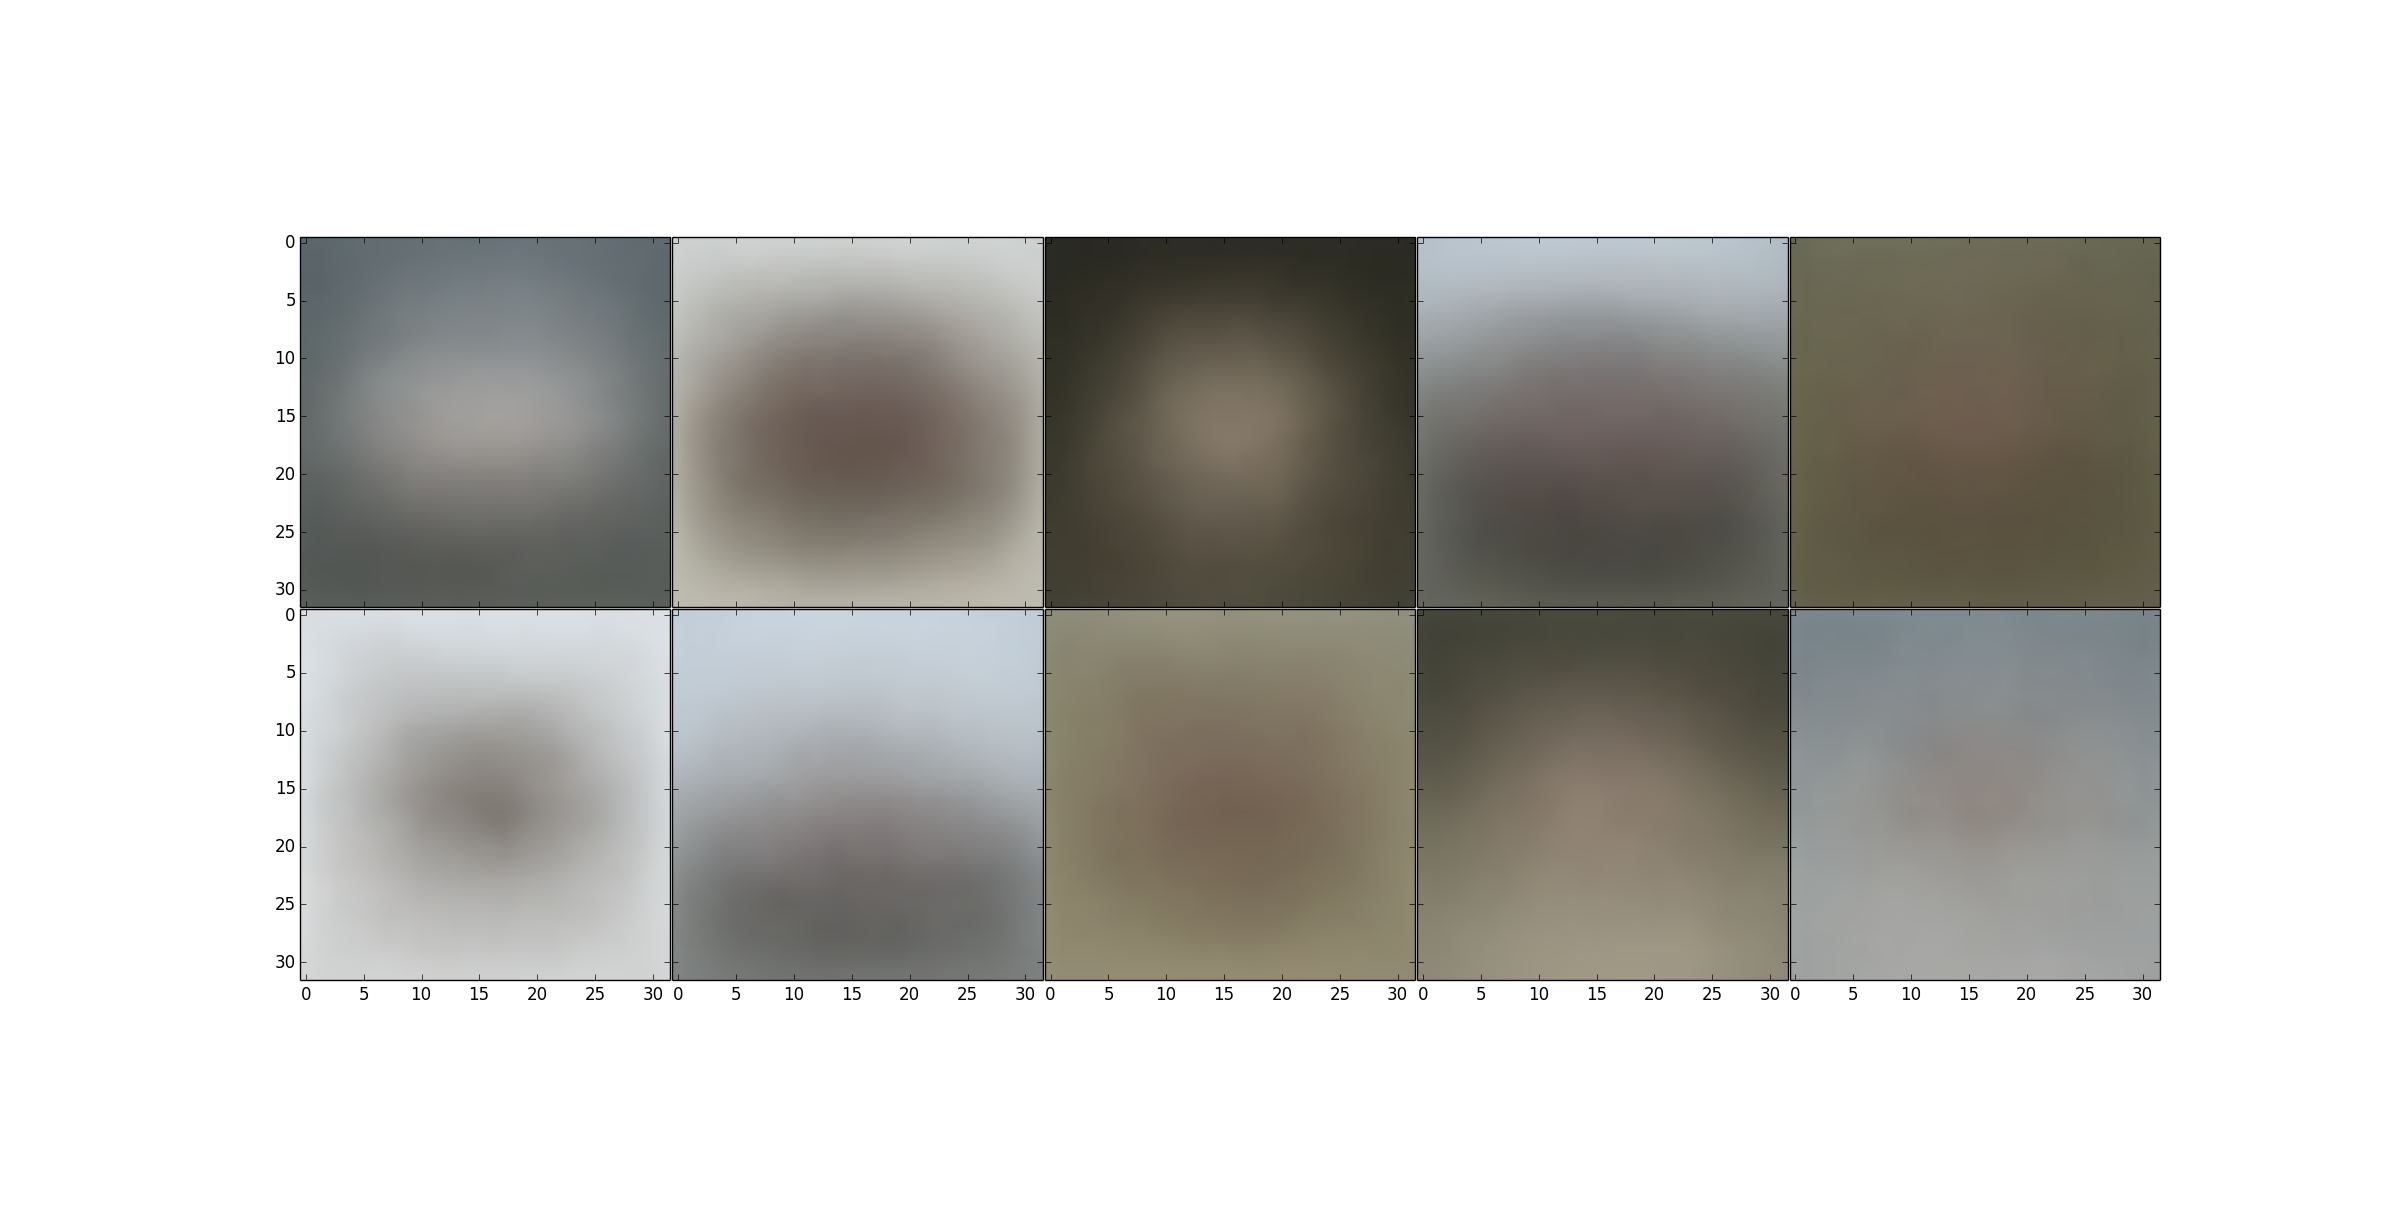
\includegraphics[width=8cm]{images/kplus10us.png}\\
	\caption{Cluster means for (top) $k=5$ and (bottom) $k=10$}
\end{figure}

We also implemented the K-Means++ algorithm. Shown below are mean images of the k clusters fo $k=5,10$. These are not qualitatively different from those of the K-Means algorithm. The objective function for $k=5$ reaches $J=2.15\times 10^{8}$, and for $k=10$ reaches $J=1.8\times 10^{8}$.

\section{Approaches for book ratings}
\subsection{K-means and K-nearest neighbor}
We first tried a preliminary approach of K-means and K-nearest neighbor. We used $K = 20$ to cluster our set of users and then predicted the book ratings based on the cluster mean. For both approaches, we standardized the user book ratings matrix by subtracting the global mean and dividing by the global variance. The predictions made with the K-means approach were almost entirely filled with 4 ratings with 3.999 and 4.0001 appearing often as well. Diagnosing our approach, we realized that the sparsity of the user book ratings matrix had essentially substituted the global mean for all unfilled spots as we clustered the users together. This meant that this approach was heavily biased towards the global mean and the results show that. The K-means approach yielded a RMSE of 0.86903, which was just slightly above the global mean.

We also attempted to use K-nearest neighbor approach where we calculated how close certain users are to each other by the number of books they have read in common and the average difference in ratings for those books. Calculating the hamming distance between users took nearly 4 hours with multiple runs due to small bugs. By that time, we decided it was more effective to pursue the probabilitistic matrix factorization approach, which, according to the Netflix competition paper, would capture unkown latent factors and be more predictive if implemented well. 

\subsection{Principal Component Analysis}
Principal component analysis (PCA) proved to be impractical for this problem because calculating the covariance matrix for the ratings was too computationally expensive, given that this is a$N\times D$ matrix where $N$ is the number of users and $D$ is the number of books.\\

An alternate approach is to use single value decomposition (SVD) to find the user-book rating matrix without having to calculate the covariance matrix. The global mean was used for imputation for empty values. However, due the the extreme sparse data, imputation resulted in most of the values in the user-book rating matrix being extremely close to the global mean.


\section{Matrix Factorization}
\subsection{Algorithm}

Given a set of ratings described by the matrix $\mat{R}$, matrix factorization attempts to decompose this into two matrices: $\mat{P}$ representing the users and $\mat{Q}$ representing the books. Each entry $\vec{p_i}$ in $\mat{P}$ represents a vector of $K$ latent features of user $i$, while $\vec{q_j}$ represents the $k$ latent factors of the book. If we can produce the matrices $\mat{P}$ and $\mat{Q}$, we can predict any entry $r_{i,j}$ in $\mat{R}$ by taking inner products of the vectors $\vec{p_i}$ and $\vec{q_j}$:
$$\hat{r}_{i,j} = \vec{p_i} \cdot \vec{q_j}^T \approx r_{i,j}$$

In the algorithm outlined by Koren et al., we iteratively train $\mat{P}$ and $\mat{Q}$ based only on the available data \cite{Koren:2009uc}.

In addition, biases are introduced to account for ratings that are dependent on either the user or the book alone \cite{Paterek:2007va,Koren:2009uc}.  Let $\mu$ be the global mean, $\vec{b}$ represent the biases for each users and $\vec{c}$ represent the biases for each book. The predicted rating is thus 
$$\hat{r}_{i,j} = \mu + b_i + c_j + \vec{p_i} \cdot \vec{q_j}^T \approx r_{i,j}$$

To learn the values of $\mat{P}$ and $\mat{Q}$, wel minimize an error function:
$$E = \sum_{i,j,r_{i,j} \in T} \left(r_{i,j} - \hat{r}_{i,j}\right)^2 + \frac{\beta}{2} \left( ||p_i||^2 + ||q_i||^2 + b_i^2 + b_j^2 \right) $$
The first term of this error function simply describes the squared reconstruction error. The second term enforces regularization---penalizing rows of $\mat{P}$ and $\mat{Q}$ that have high magnitude. 

We use $\nabla e_{i,j}$, the gradient , to minimize $e_{i,j}$ (and hence $E$) by stochastic gradient descent.

\begin{align*}
p_{i,k} &\gets p_{i,k} + \alpha \left(2 \left(r_{i,j} - \hat{r}_{i,j}\right)  q_{j,k} - \beta p_{i,k} \right) \\
q_{j,k} &\gets p_{i,k} + \alpha \left(2 \left(r_{i,j} - \hat{r}_{i,j}\right)  p_{i,k} - \beta q_{j,k} \right) \\
b_{i}   &\gets p_{i,k} + \alpha \left(2 \left(r_{i,j} - \hat{r}_{i,j}\right)          + \beta b_{i}   \right) \\
c_{j}   &\gets p_{i,k} + \alpha \left(2 \left(r_{i,j} - \hat{r}_{i,j}\right)          + \beta c_{j}   \right)
\end{align*}

We update $\vec{p_i}$, $\vec{q_j}$, $b{i}$, and $c_{j}$ for each pair $(i, j, r_{i,j}) \in T$. This process is repeated for some number of steps, or \emph{epochs}, until either some criterion for epochs is met (e.g. the change in the total error $E$ is less than some $\epsilon$, or the maximum number of epochs is exceeded). 

\subsection{Optimization}
The main issue we had with the matrix factorization approach was that there were many of meta-parameters to tune: the learning rate $\alpha$, the regularization parameter $\beta$, the number of latent factors $K$, and the criteria for determining convergence. We estimated appropriate starting values for $K = 5$ and $\beta = 0.02$ based on literature on the Netflix prize \cite{Mnih:2007wg,Ott:2008tu}, and we experimented to determine that $\alpha = 0.001$ generally produced convergent solutions. We tried the following reductionist methods for validating our approach, and for further tuning these parameters:

\begin{enumerate}
\item Checking the gradient. We verified that our gradient function was correct by finite differences.
\item Recapitulating the user mean results. We tried setting $K=1$, $\beta=0$ and fixing $q_{j,k} = 1$. This gave us an RMSE of 0.77857---slightly better than the user mean results. However, when $q_{j,k}$ is not fixed, the RMSE is greater than 1, which points to an instability in the algorithm.
\item Reconstruction of fake data. We generated fake values for $\mat{P}$ and $\mat{Q}$, and multiplied them together to get a fake $\mat{R}$. We then trained the model on $T$ containing some fraction of the $r_{i,j}$'s.  
\item Cross-validation. We withheld a subset (between 1--10\%) of our training data, trained the model on the remainder, computed the difference between the predicted ratings and the withheld ratings. We used this method to attempt to set our parameter.
\item Tests were run using both standardized data, in which the ratings are scaled such that mean is 0 and standard deviation is 1, and non-standardized data.
\item Ranging $k=1$ to 3 and calculating the RMSE on the withheld data shows a trend of increasing RMSE with $k$. However, these results are not valid given that $k=1$ does not give positive results.
 
\end{enumerate}

\subsection{Results and Conclusion}
We achieved our best RMSE value of 0.77857 with the probabilistic matrix factorization approach that the winners of the Netflix competition used. This was with latent factor $K = 1$, $\alpha = 0.001$, and $\beta = 0.0$, with no bias vectors. As noted, this is slightly better than the user mean RMSE value. 

Increasing the number of latent factors seemed to make the results worse. Likewise, adding in the bias vectors or increasing $\beta$ also seemed to be detrimental to the results. This observation might be explained by the overfitting of the sparse data set. Having too many factors to learn from the training set causes the machine learning algorithm to overfit the training data and perform less optimally on the test set.


\bibliography{library}
\bibliographystyle{ieeetr}


\end{document}  
